%%%%%%%%%%%%%%%%%%%%%%%%%%%%%%%%
\section{The application of the `Geber' method}
\label{app:gpe2}
%%%%%%%%%%%%%%%%%%%%%%%%%%%%%%%%
In this section, we provide more information on the applied genotype-phenotype-environment equation \parencite{Ellner2011,Hairston2005}, this is the variant of the `Geber' method that \cite{Ellner2011} developed and forms the basis of our analysis. First, we describe the method in more detail. This framework was applied to each simulated dataset.

\subsection{The method} \label{app:gpe2:eq}
In our analysis, we have followed the example described in \cite{Ellner2011} on great tits to quantify the contribution of the three processes in influencing average body size $\overline z$ in the population. This version depends on two steps. 

First, we fitted a linear model to estimate the effects of average breeding value ($\overline a$), average plasticity at birth ($\overline p$) and average consumed food ($\overline k$) on the average trait value ($\overline z$). 

We then used separate regressions of each of the three factors on time to predict their values at the beginning ($t=11$) and at the end of the interval ($t^\prime=50$). Using these predicted values, together with the model for $z$, we estimated $\hat z$ at time $t$ (=$\hat z(\hat{a}_t,\hat{p}_t,\hat{k}_t)$) and at time $t^\prime$ (=$\hat{z}(\hat{a}_{t^\prime},\hat{p}_{t^\prime},\hat{k}_{t^\prime})$). We then predicted the change in $\hat{z}$ for mixed scenarios, where one or two factors were estimated at time $t$ and the remaining factor(s) at time $t^\prime$ (e.g. $z(\hat{a}_{t^\prime},\hat{p}_{t},\hat{k}_{t})$). We used all eight ($2^3$) combinations of the three factors at either time point and regressed the so obtained eight values of $\hat z$ on three binary dummy variables (one for each factor, indicating which of the values of the corresponding factor was used for the calculation of $z$). The coefficients of this regression provided the relative contributions of the three factors.

\subsection{Using genotypic values from the simulation}\label{app:elln:bvs}
When genotypic values from the simulations were used instead of breeding value estimates by the AM, we obtain the result shown in Figure \ref{fig:gpeGV}. We see that now the bias in the evolutionary components has disappeared and that the plasticity component is in line with the expectation as outlined in the main text (i.e. small but negative, due to a slight decrease in average maternal body size weighted by litter size over time.).
\begin{figure}[b]
\centering
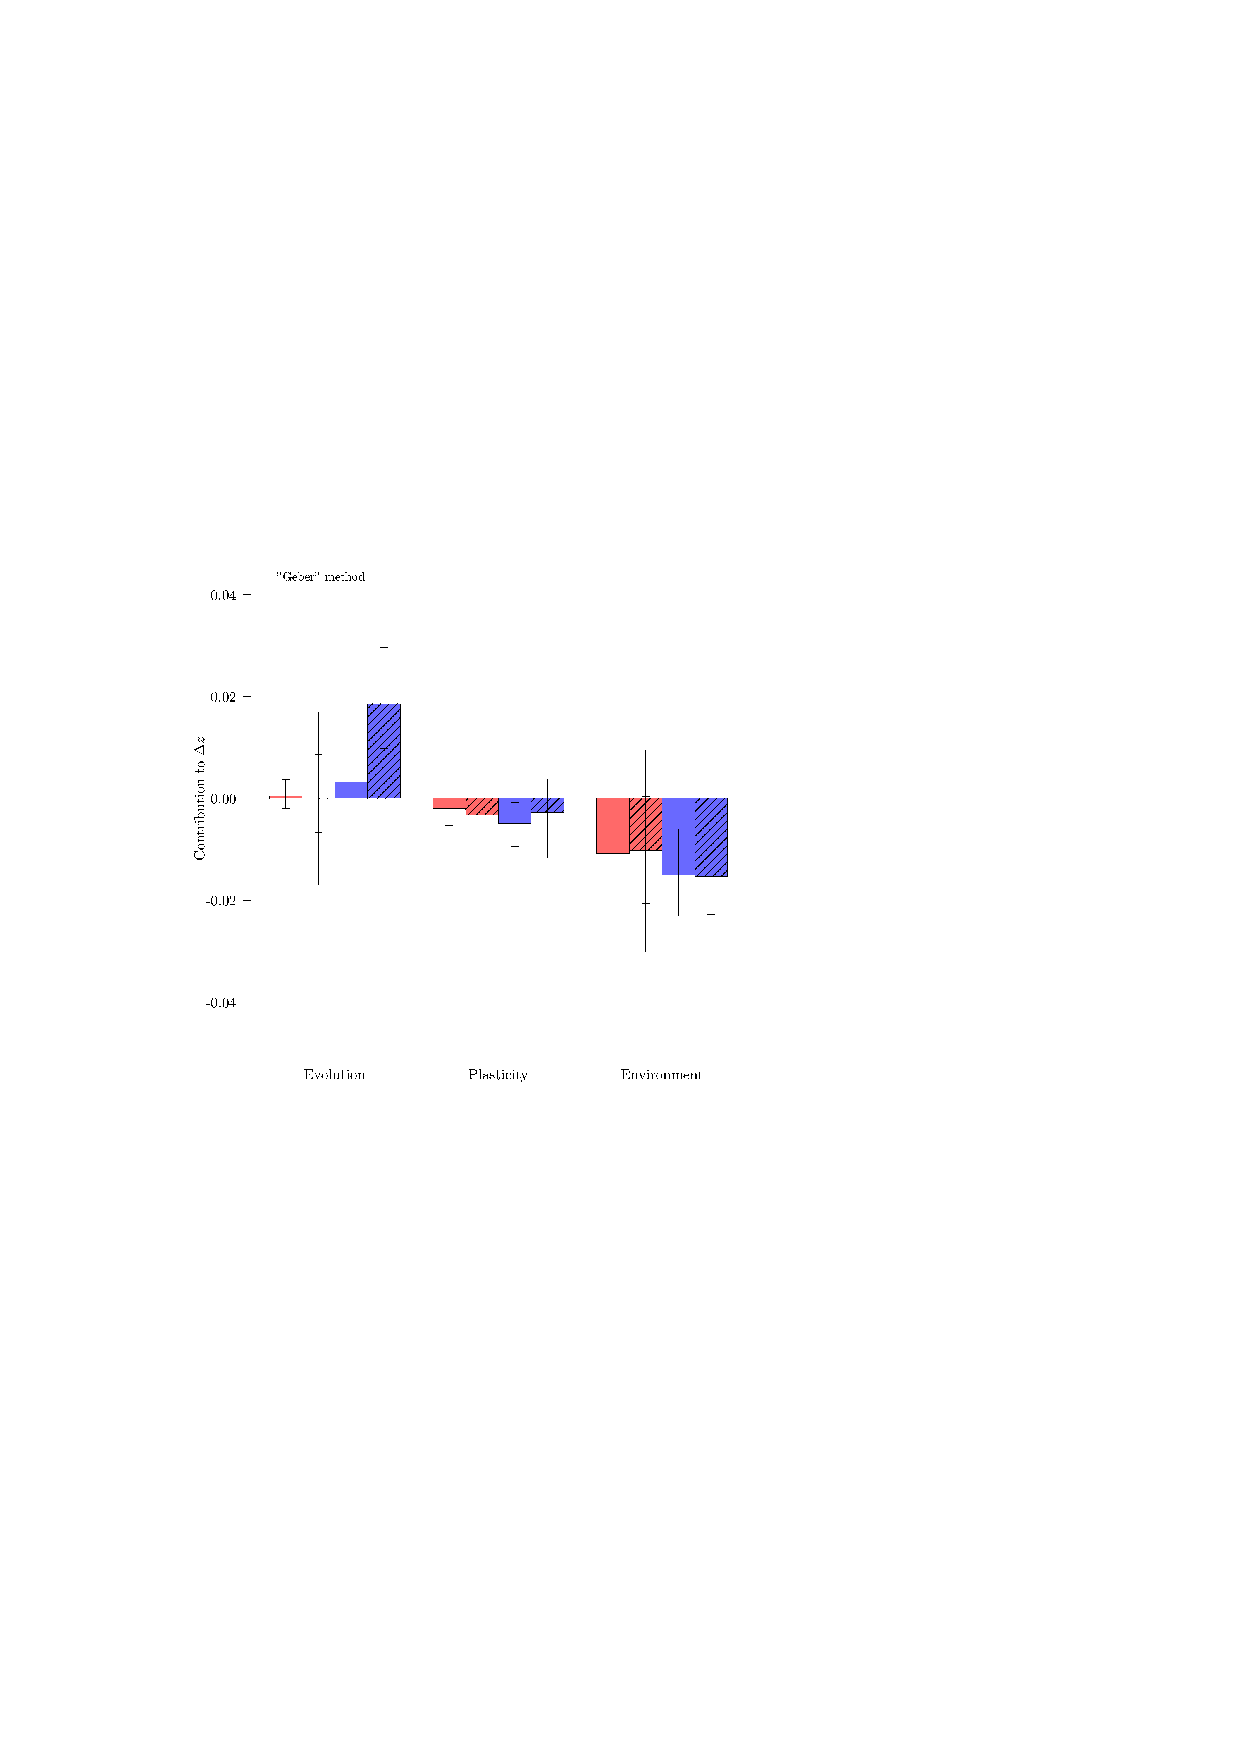
\includegraphics[width=0.65\textwidth]{Appendices/FigS4}
\caption{\footnotesize Results of the GM when based on the actual (simulated) genotypic values instead of on the estimated breeding values.}
\label{fig:gpeGV}
\end{figure}
